\documentclass{beamer}

\usetheme[]{Rochester}
\usecolortheme{beaver}
\usepackage[latin1]{inputenc}
\usepackage{graphics}

\author{Will Webberley}
\date{Autumn 2014}
\institute[COMSC]{Cardiff School of Computer Science and Informatics}



\title{Task Analysis}
\subtitle{CM2101: Human-Computer Interaction}

\begin{document}

\frame{\titlepage}

\frame{
    \frametitle{Task analysis}
    \center{
        The analysis of tasks that users carry out on a system 
    }
    \vskip20pt
    \flushleft{
        \textbf{Essentially, task analysis asks...}
        \begin{itemize}
            \item What needs to be done?
            \begin{itemize}
                \item A `goal'
            \end{itemize}
            \item What needs to be done \textit{beforehand}?
            \begin{itemize}
                \item Preconditions
                \begin{itemize}
                    \item Other tasks that this goal \alert{depends on}
                    \item \alert{Prior knowledge} the user needs
                \end{itemize}
            \end{itemize}
            \item What \textit{steps} are involved in completing the goal?
            \begin{itemize}
                \item Are there any \alert{subtasks}?
                \item Often, these can be \alert{decomposed recursively}
            \end{itemize}
        \end{itemize}
    }
}

\frame{
    \frametitle{Task analysis}
    \begin{itemize}
        \item Specify task structure
        \item More detailed interaction with a user interface
        \item Helps ullustrate \alert{architectural issues} in interactive systems
        \item Helps as a pre-design tool to compute a series of steps to complete a goal
        \item Many task structures are \alert{hierarchical}
        \item We need to consider \alert{system tasks} as well as user tasks
    \end{itemize}
}
    
\frame{
    \frametitle{Task analysis in evaluation}
    \textbf{Task analysis generally ties in quite deeply to GOMS and KLM}
    \vskip10pt
    \begin{columns}
        \column{.5\textwidth}
            \begin{itemize}
                \item How complex is a task?
                \item How many \alert{steps} does the task involve?
                \item Which \textit{cognitive} \alert{operators} does it involve?
                \item Which \textit{motor} operators does it involve?
                \item Is there more than one \alert{method} to complete the task
                \item Use \alert{selection} rules to choose between them 
            \end{itemize}
        \column{.5\textwidth}
            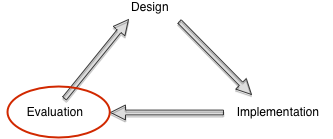
\includegraphics[width=5cm]{media/cycle_2.png}    
    \end{columns}
}

\frame{
    \frametitle{Task analysis in design}
    \textbf{Again, with the help of GOMS and KLM...}    
    \vskip10pt
    \begin{columns}
        \column{.5\textwidth}
            \begin{itemize}
                \item Which controls need to be included?
                \item Where should controls be placed?
                \item Which parts of the system are most accessible?
                \item How big should the buttons be?
                \item Which options should be on action bars? Which should be in menus?
                \item etc.
            \end{itemize}    
        \column{.5\textwidth}
            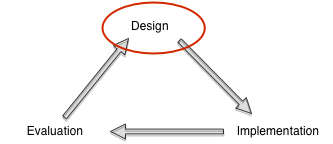
\includegraphics[width=5cm]{media/cycle_3.png}
    \end{columns}
}

\frame{
    \frametitle{Aspects of task analysis}
    \begin{columns}
        \column{.6\textwidth}
            \begin{itemize}
                \item \textbf{User model} 
                \begin{itemize}
                    \item Users' mental image of system objects
                    \item Tasks in mind
                \end{itemize}
                \item \textbf{Designer model}
                \begin{itemize}
                    \item Designer's idea of system objects
                    \item Knows what actions can be performed
                    \item Knows what information is associated with which objects
                    \item Knows what the relationship between objects is
                \end{itemize}
            \end{itemize}  
        \column{.4\textwidth}
            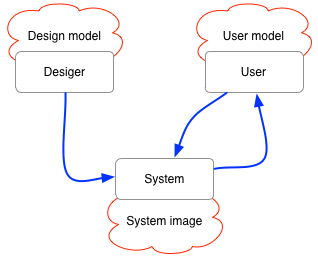
\includegraphics[width=5cm]{media/models.png}
    \end{columns}
    \begin{itemize}
        \item \textbf{System image}
        \begin{itemize}
            \item Mental model derived from interaction with system
            \item The way designers communicate with users
        \end{itemize}
    \end{itemize}
} 

\frame{
    \frametitle{Theory of action}
    \textbf{The states are separate}
    \vskip15pt 
    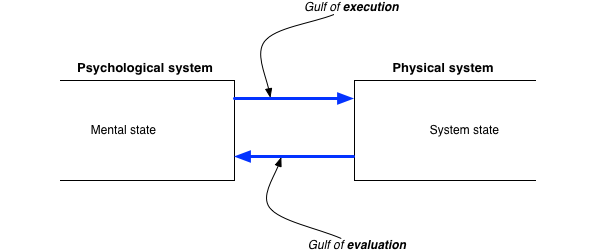
\includegraphics[width=\textwidth]{media/gulfs.png}
}

\frame{
    \frametitle{Theory of action}
    \textbf{Gulf of \alert{execution}}\\
    Distance between the user's \alert{goals} and the means of \alert{achieving} them through the system
    \vskip30pt
    \textbf{Gulf of \alert{evaluation}}\\
    Amount of effort required to determine the system state. Did the system do what the user wanted?
}

\frame{
    \frametitle{Theory of action}
    \textbf{The gulfs can be  \alert{bridged}}\\
    \center{
        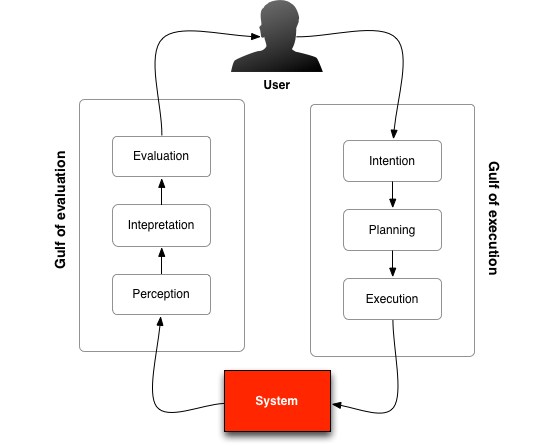
\includegraphics[width=8cm]{media/gulfs_2.png}
    }
}

\frame{
    \frametitle{Applying task analysis}
    \textbf{Consider the `bridges' when conducting task analysis}
    \vskip15pt
    \begin{itemize}
        \item Consider the \textit{learnability} of the system
        \item Consider the \textit{Memorability} of the system
        \item Reduce the amount of \alert{cognitive} power required in gulfs
        \item Reduce the amount of \alert{time} required to perform tasks
        \vskip20pt
        \item For example, could you design a task such that:
        \begin{itemize}
            \item the \alert{planning} time is reduced?
            \item the \alert{interpretation} is less complicated?
            \item the \alert{intentions} are easier to form (through improving \textit{Visibility})
        \end{itemize}
    \end{itemize}
}

\frame{
    \frametitle{Task design}
    \begin{itemize}
        \item Task design:
        \begin{itemize}
            \item Review functional requirements carefully
            \item Ensure system (hardware, software) can support task goals
        \end{itemize}
        \vskip20pt
        \item Consider:
        \begin{itemize}
            \item \alert{Goal}: the final state
            \item \alert[Sub-goals}: sub-states required to achieve main goal
            \item \alert{Action}: a task that requires no problem-solving or control structure
            \item \alert{Dialogue}: occurs to bind actions together to achieve a (sub-)goal        
        \end{itemize}
    \end{itemize}
}



\frame{
    \frametitle{Hierarchical task analysis}
    \textbf{Aims}
    \begin{itemize}
        \item \alert{Describe} the task as a goal to be reached
        \item Find conditions under which sub-goals should be executed
    }
    \textbf{Involves}
    \begin{itemize}
        \item \alert{Identifying} tasks
        \item \alert{Breaking} down into sub-tasks
        \item Checking \alert{accuracy} of decomposition
        \item Usually represented \alert{graphically}
    \end{itemize}

    \textbf{Clearly shows...}
    \begin{itemize}
        \item The top-level \alert{goals}
        \item How the goal is recursively decomposed into \alert{sub-goals}
        \item Low-level \alert{actions}
        \item \alert{Dialogue} represented by the \textit{order} of actions
    \end{itemize}
}

\frame{
    \frametitle{Conducting a task analysis}
    \textbf{4 main steps}
    \begin{enumerate}
        \item \alert{Collect data} on current tasks
        \item Represent in an appropriate \alert{notation}
        \item \alert{Generalise} across tasks
        \item Apply in \alert{design}
    \end{itemize}
}

\frame{
    \frametitle{Task design: 1. Collect data}
    \begin{itemize}
        \item Refer to documentation
        \begin{itemize}
            \item What tasks need to be done?            
        \end{itemize} 
        \item Ethnography (i.e. studying users)
        \begin{itemize}
            \item How do users carry out their tasks?
        \end{itemize}
        \item User reports (interviews or questionnaires)
        \begin{itemize}
            \item How do users \textit{currently} carry out tasks?
            \item How \textit{often} are they performed?
            \item \textit{Where} are tasks performed?
            \item What information needs to be handled in the tasks?
        \end{itemize} 
    \end{itemize}     
    Designer's aim is to make tasks feel natural and more \textit{usable} for users.
}

\frame{
    \frametitle{Task design: 2. Represent in notation}
    \textbf{We consider \alert{Jackson Structured Development} as notation} 
    \begin{columns}
        \column{.5\textwidth}
            \begin{itemize}
                \item Type of hierarchical task analysis 
                \item Captures:
                \begin{itemize}
                    \item Iteration (`*')
                    \item Alternatives ('o')
                    \item Task-ordering relationships
                \end{itemize}
                \item Components:
                \begin{itemize}
                    \item Box - task description
                    \item Hierarchy - Decomposition and order
                    \item Box colour code - user task, system task, shared task
                \end{itemize}
            \end{itemize}
        \column{.5\textwidth}                
            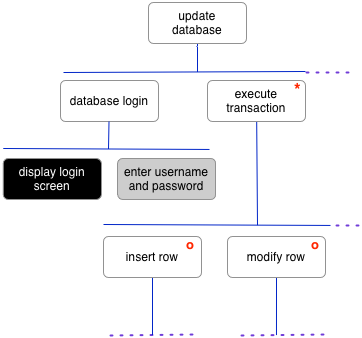
\includegraphics[width=5cm]{media/jackson_1.png}
    \end{columns}
}

\frame{
    \frametitle{Task design: 2. Represent in notation}
    \textbf{Jackson Structured Development}
    \begin{itemize}
        \item Easily see major tasks
        \item Also easily see how each task can be decomposed
        \item Up to designer or evaluator how detailed to go
        \item Can be used to supplement GOMS or KLM, if needed
        \item Traditional use-cases only address a user's interaction with system...
        \item ... JSD allows for perceiving the full context of a task's execution
    \end{itemize}
}

\frame{
    \frametitle{Jackson Structured Development: example}
    \textbf{\alert{Stage 1}: Break down task for \textit{user}- e.g. a drink vending machine}
    \vskip20pt
    \begin{enumerate}
        \item Select drink type
        \item Select option (milk or cream)
        \item Select option (sugar)
        \item Pay
    \end{enumerate}
}

\frame{
    \frametitle{Jackson Structured Development: example}
    \textbf{\alert{Stage 2}: Identify sub-tasks, \textit{system} tasks, and visualise}
    \vskip20pt
    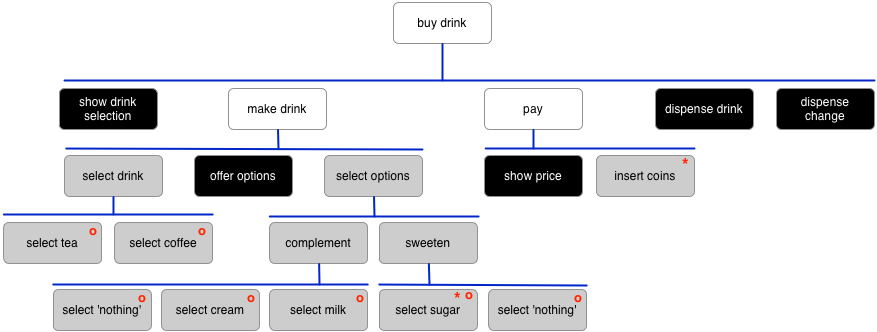
\includegraphics[width=\textwidth]{media/jackson_2.png}
}

\frame{
    \frametitle{Uses of Jackson notation}
    \begin{columns}
        \column{.5\textwidth}
            \textbf{In `evaluation'}
            \begin{itemize}
                \item Allows experts to \alert{describe} tasks
                \item Allows for \alert{errors} or \alert{omissions} in flows to be identified
                \item Allows evaluation against original \alert{requirements}
                \item Ensures each task can be completed
            \end{itemize}
        \column{.5\textwidth}
            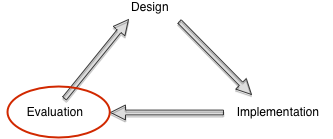
\includegraphics[width=5cm]{media/cycle_2.png}
    \end{columns}
}

\frame{
    \frametitle{Uses of Jackson notation}
    \begin{columns}
        \column{.5\textwidth}
            \textbf{In `design'}
            \begin{itemize}
                \item Helps identify \alert{shared tasks} between user and system
                \item Helps find where \alert{feedback} might be necessary
                \item Task ordering helps design \alert{dialogues}
            \end{itemize}
        \column{.5\textwidth}
            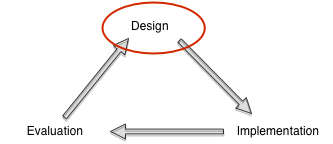
\includegraphics[width=5cm]{media/cycle_3.png}
    \end{columns}
}

\frame{
    \frametitle{Task design: 3. Generalise}
    \begin{itemize}
        \item Find common sub-goals across primary goals
        \begin{itemize}
            \item Can these be duplicated to help improve \textit{Learnability}?
        \end{itemize}   
        \item Refer to data-collection to stage to see which tasks are performed frequently
        \item Frequent tasks should be `easy' to perform
        \item What is the effect on ordering of events?
    \end{itemize}
}

\frame{
    \frametitle{Task design: 4. Apply in design}

}

\frame{
     \frametitle{Revision questions}
     \begin{enumerate}
        \item
     \end{enumerate}
}

\frame{
    \frametitle{Summary}
    \begin{itemize}
        \item 
    \end{itemize}
}    




\end{document}
